%!TEX root = main.tex
\newpage
\thispagestyle{empty}
\mbox{}
\chapter{PeacefulBanana Quick Start}

\begin{figure}[h!]
\label{logo}
\centering
	
\includegraphics[width=\textwidth]{logo}
\caption{PeacefulBanana Reflection tool}
\end{figure}

This chapter features the PeacefulBanana quick start guide, given to the students for our evaluation. \\
Peaceful Banana is a tool aimed towards aiding reflection in teams. It integrates with GitHub, collects the most relevant project artifacts and scaffolds these in order to trigger and promote reflection in your team.
See you and your co-workers latest activity and use tag-cloud or statistics to create your daily reflection notes. PeacefulBanana allows you to choose what to share, and what to keep private! Reflect on your individual work by revisiting reflection notes, or reflect on your team's activity through reflection workshops and much more. 
\pagebreak

\section{Getting started}
So you and your team are developing software, using an agile process model? In that case you are probably familiar with the aspect of reflection or retrospectives in agile methods. The purpose of these retrospectives after each iteration is mainly to learn what works and what does not work, in order to make adjustments for the next iteration. More specifically your team wants to answer two fundamental questions:
\begin{itemize}
\item What went well during the last iteration that we continue doing? 
\item What could we do differently to improve?
\end{itemize}

The PeacefulBanana tool can help you and your team to identify the common ground answers to these questions. But first, we need to ensure you have the tools needed to use PeacefulBanana: \\
In order to use the Peaceful Banana application you need access to a device with an up-to-date internet browser, such as Firefox, Google Chrome, Safari, Opera or Internet Explorer(version 7 and up). Other browsers present on tablets and smartphones may also work, but we suggest using one of the mentioned here. \\
That's it! That is all you need to have in order to begin using PeacefulBanana. 
In order to access the web-application, you need to open your browser and access this url: \url{http://vm-6121.idi.ntnu.no:8080/PeacefulBanana/} . Here you will be greeted by our welcome screen\\

\begin{figure}[h!]
\label{homescreen}
\centering
	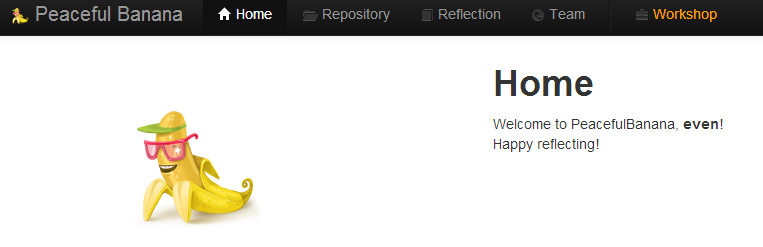
\includegraphics[width=\textwidth]{home}
\caption{PeacefulBanana Landing Screen}
\end{figure}

\pagebreak
\subsection{Registration}
In order to become part of the PeacefulBanana community, you need to register for a new account. To do this, click the login button in the top right corner. At the login screen press the 
\textit{Not yet a user?} link, as shown here:
\begin{figure}[h!]
\label{login}
\centering
	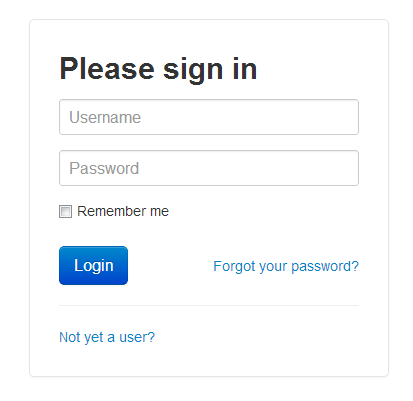
\includegraphics[width=\textwidth]{login}
\caption{PeacefulBanana Login screen}
\end{figure}

After filling in your registration details, you will receive an email containing a confirmation link. By clicking this link you will automatically be logged in to PeacefulBanana and redirected to GitHub for authorization. 
In order for PeacefulBanana to collect necessary data from GitHub, you will need to authorize our application, this will look something like this: 

\begin{figure}[h!]
\label{authorize}
\centering
	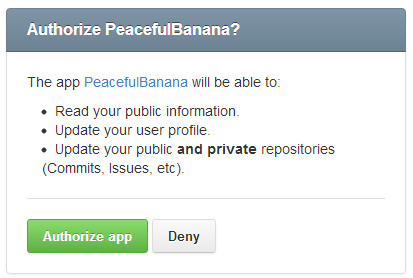
\includegraphics[width=\textwidth]{authorize}
\caption{PeacefulBanana - GitHub application authorization}
\end{figure}

This registration and authorization is only a one-time process. When you have registered and authorized the PeacefulBanana application, you won't need to do think about it again. We'll take care of the rest. 
\pagebreak

%
%TEAM TAB
%
\subsection{Choosing team}
Now you are ready to explore what PeacefulBanana can offer you and your team. The first screen you will see is the team screen:

\begin{figure}[h!]
\label{teamscreen}
\centering
	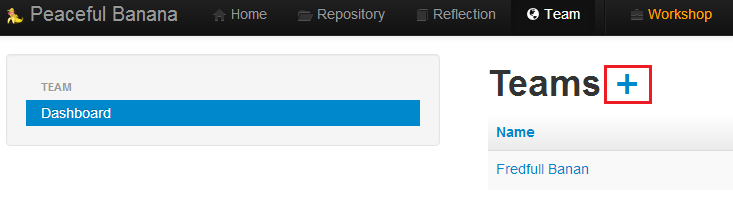
\includegraphics[width=\textwidth]{teamscreenquickstart}
\caption{PeacefulBanana - Team page, currently no teams have been created}
\end{figure}

The first thing you have to do is get the team leader to create a new team. One PeacefulBanana team retrieves data from your chosen GitHub repository and only that. All repository collaborators can join the PeacefulBanana team, so if you are having trouble joining the team - check if you have the collaborator status on the GitHub repository. Creating a team can be done simply by clicking the highlighted \emph{+}\\
On the next screen, choose a suitable team name and which repository this team should be linked to. As stated earlier, there can only be one team for each repository, and only the team leader needs to create the team. After clicking \textit{Create} PeacefulBanana will working it's magic and retrieve your chosen repositories' data. This includes commits, milestones, issues you are already familiar with on GitHub. This process might take a while the first time around, but don't worry, you will be notified when this process is complete.\\
Back at the team page, your team will be created and visible under \emph{Teams}. Also the newly created team will be available to join for the other team members. Go ahead and invite your co-collaborators to join!
\begin{figure}[h!]
\label{teamcreated}
\centering
	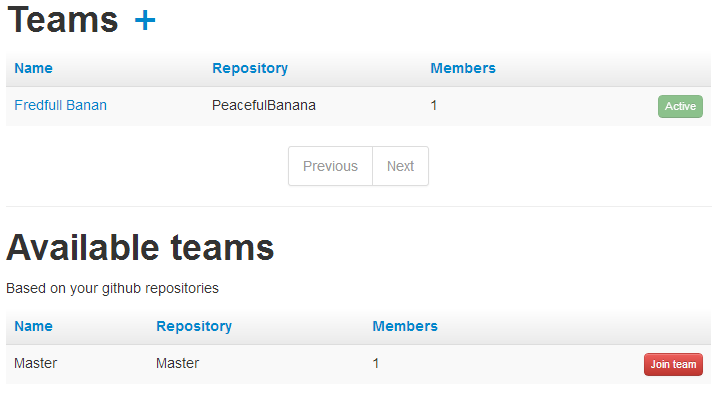
\includegraphics[width=\textwidth]{teamcreated}
\caption{PeacefulBanana - Team page showing current team and available teams based on your repositories}
\end{figure}

%
% Repository TAB - Sell sell sell!
%

\subsection{Repository tab}
Clicking the repository tab, you will be presented with a screen like this:
\begin{figure}[h!]
\label{repository}
\centering
	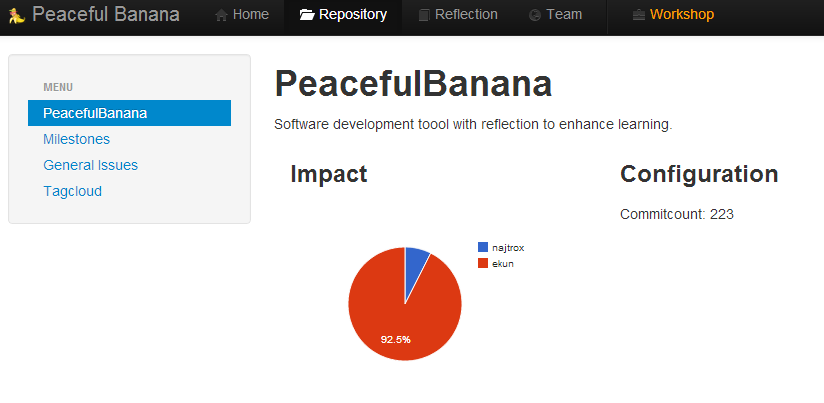
\includegraphics[width=\textwidth]{Repositorymenu}
\caption{PeacefulBanana - The main repository screen}
\end{figure}
\\
It's a simple start screen with the overall commit impact for your team's repository and a commit count. This information can be used to gain an indication of who is having the largest impact in the current team and how much overall activity there is. 
On the menu to the left you can see tabs for your repositories' milestones, issues and tagcloud.
\\
\textbf{The milestones sub-tab:}
\begin{figure}[h!]
\label{milestones}
\centering
	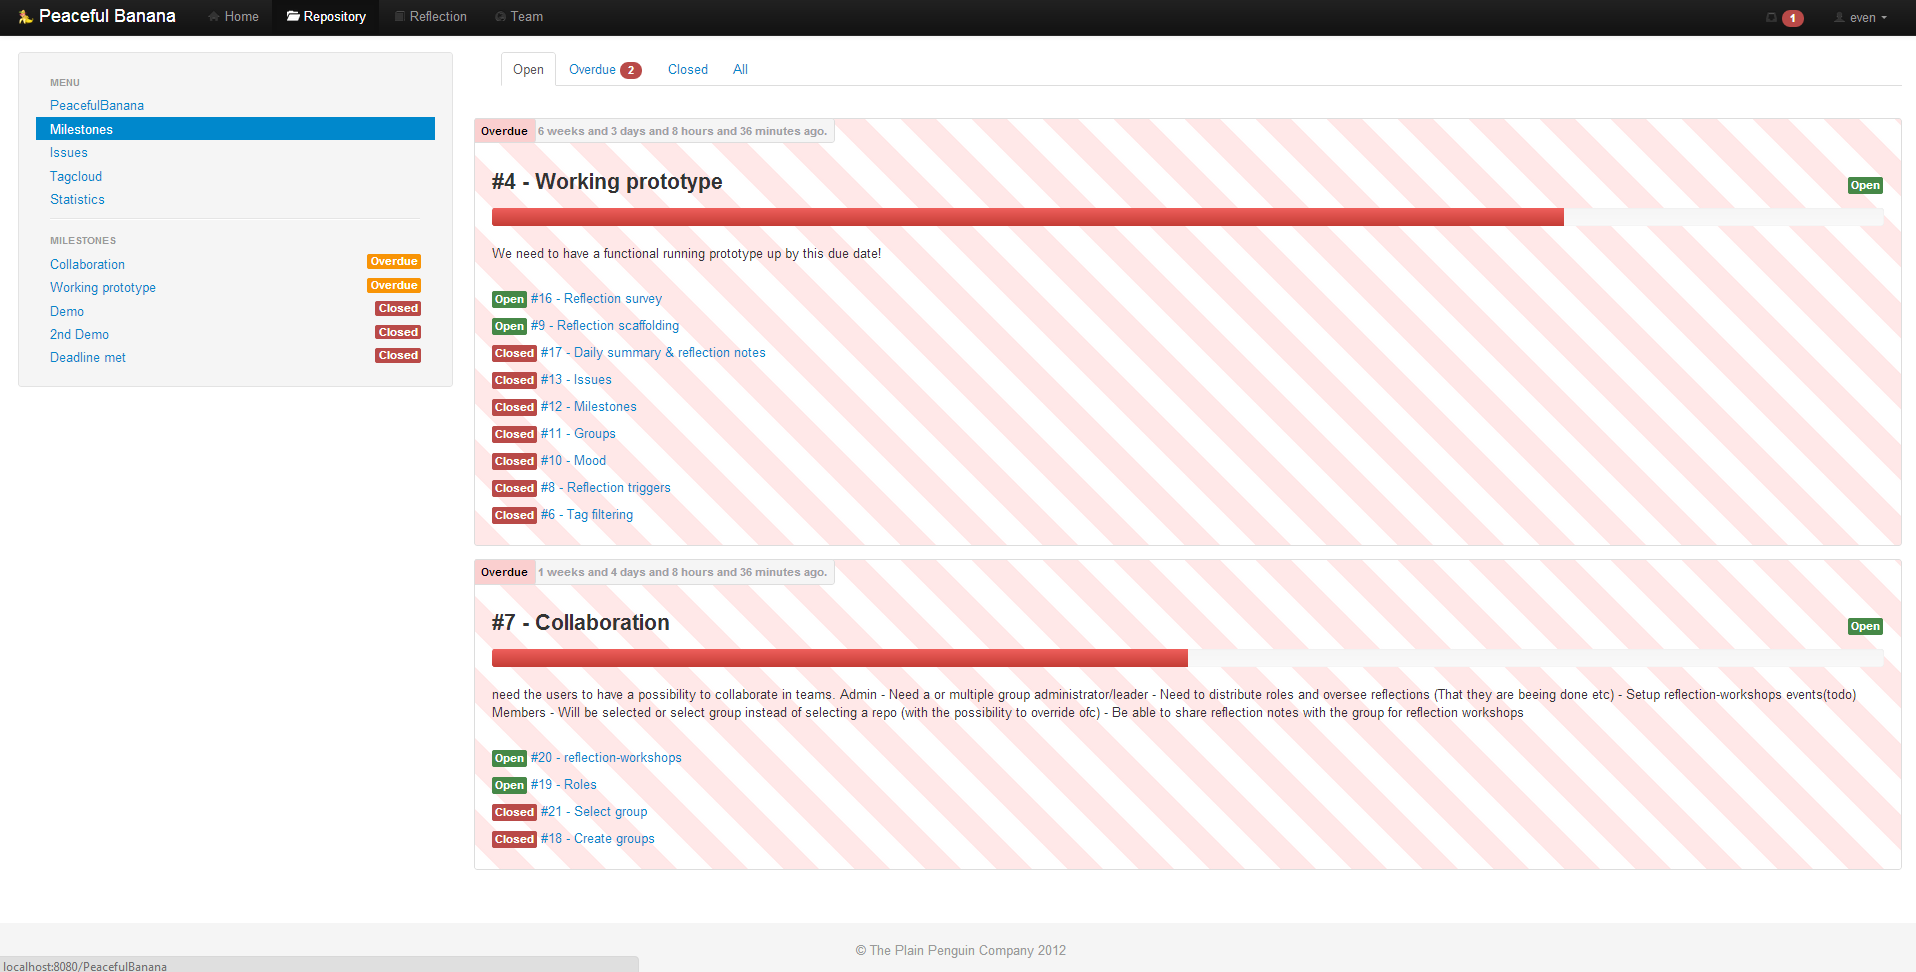
\includegraphics[width=\textwidth]{milestones_full}
\caption{PeacefulBanana - All the repositories' milestones}
\end{figure}
\newpage
On the milestones sub-menu you have access to all your milestones and their status(Open, Overdue or Closed). The main tab will by default show all your Open milestones. At the top you can switch to see milestones with other statuses.\\
It's fast and easy to switch between your currently open milestones,the ones that are overdue and the milestones you already have closed. This functionality makes it useful for individual daily usage, and for preperation to team retrospectives. Say your team missed an important deadline, and you wish to dive into what issues were causing problems. Clicking on this milestone will present you with all the issues that are connected to that milestone, in a clean manner:
\begin{figure}[h!]
\label{milestonessingular}
\centering
	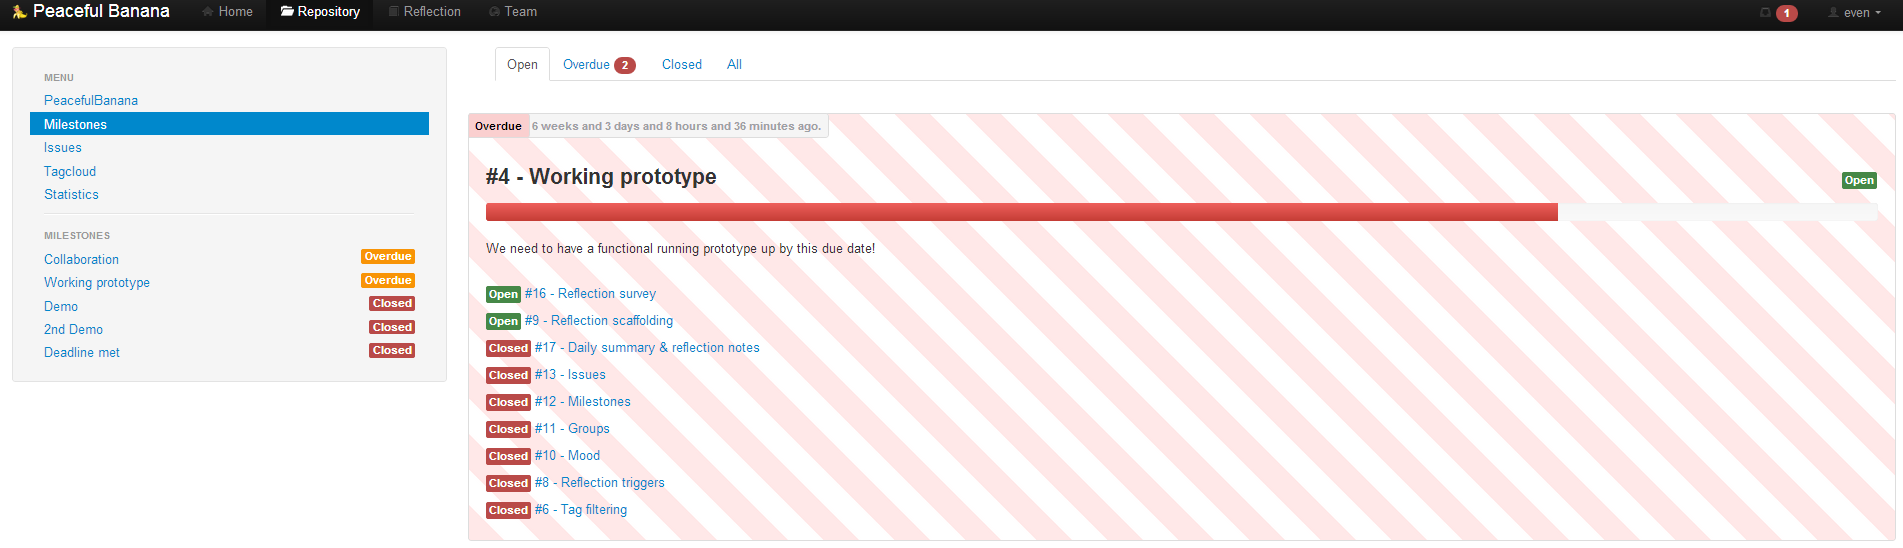
\includegraphics[width=\textwidth]{milestone_medium}
\caption{PeacefulBanana - Single milestone}
\end{figure}
PeacefulBanana shows you that particular milestone's issues and their status, in addition to a milestone specific tagcloud. This tagcloud will help you identify which tags\footnote{\# prepended words in commit-messages} are the most active, related to this particular milestone. This will in turn identify which issues might be worth taking a closer look at, while excluding the less important ones. 
Say if you see that issue \#20 has been heavily referenced in commits, and you want to see further details surrounding that issue, simply click it:
\begin{figure}[h!]
\label{milestonessingular}
\centering
	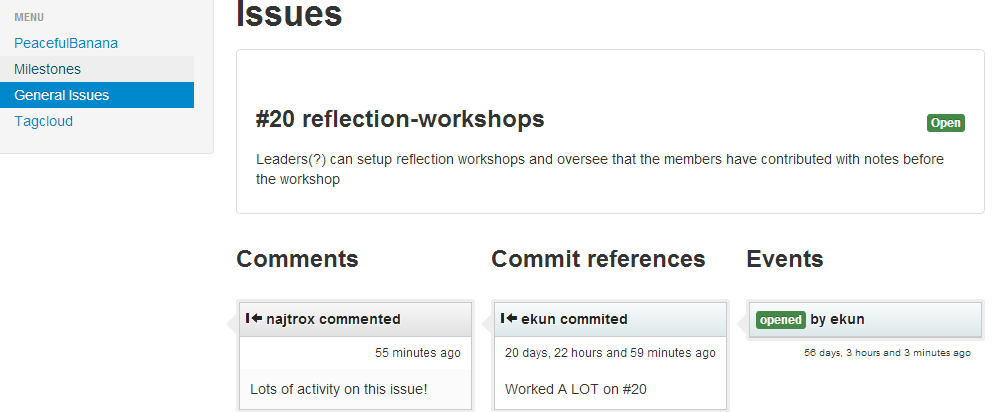
\includegraphics[width=\textwidth]{issue20small}
\caption{PeacefulBanana - Issue \#20, listing comments, references and events}
\end{figure}
PeacefulBanana shows you this issue's comments, references and events all in one clean interface, so that you or your team can quickly identify the activities. 

%
% Reflection tab
%

\subsection{Reflection \& Reflection notes}
A typical scenario in retrospectives, is that it's often hard to recollect all events for the last two-three weeks. PeacefulBanana aims to remove this issue completely from the retrospective sessions.\\*
The reflection tab contains your personal reflection notes, and also your team's shared reflection notes. After creating a personal note, you can choose to share one or more of these with your team. It is not shared by default, so your personal notes really are personal. It is encouraged to share reflection notes with the team, the more notes shared - the easier it is to find common improvements and difficulties in the team. Personal notes may be used by you for personal reflection, or as preparation for a team retrospective meeting. The shared notes can be used by the team during the retrospective meeting.\\
\begin{figure}[h!]
\label{milestonessingular}
\centering
	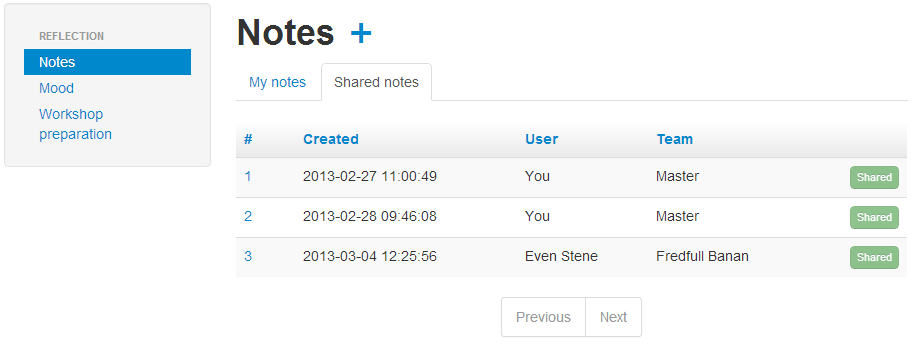
\includegraphics[width=\textwidth]{notes_shared}
\caption{PeacefulBanana - Reflection tab with the currently shared notes}
\end{figure}
PeacefulBanana also provides you and your team with a mood-graph under the tab \textit{Mood}, which ranges from members beeing very happy, to very sad. This moodgraph will give you and your team an indication of how the individual moods progressed through the project. Is there any specific period where the team's mood ranged a lot? Then this period would be worth having a second look, as to what exactly was beeing worked on at the time, any specific problems or issues that could have been avoided?\\

Another feature of PeacefulBanana is the the tab \textit{Workshop Preparation}, which helps users prepare for the team's retrospective sessions. You can easily switch between created workshops, and see your individual notes created for that particular workshops'. Revisiting these contributions and improvements helps users recollect the experiences from the particular days, the daily contributions and improvements, and finally that periods moodgraph for both you and your team.\\*
\begin{figure}[h!]
\label{milestonessingular}
\centering
	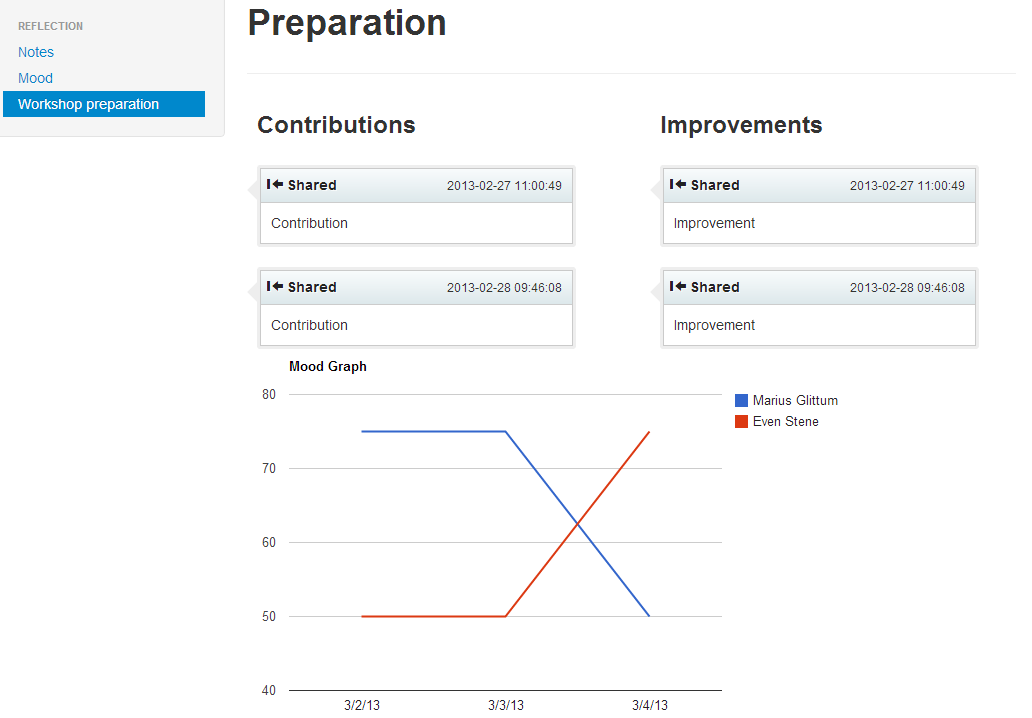
\includegraphics[width=\textwidth]{workshop_prep}
\caption{PeacefulBanana - Reflection tab with the currently shared notes}
\end{figure}

%
% Workshop tab
%

\subsection{Workshop tab}
Finally we have the workshop tab. This is only visible if you are the manager of your current active team. This means that only the team leader can create workshops. 
If you wish to create a new workshop, simply click the + icon next to the title: 
\begin{figure}[h!]
\label{workshop_plus}
\centering
	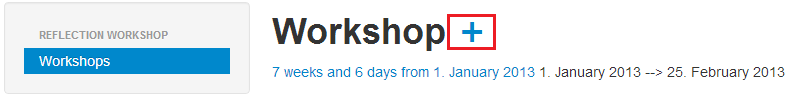
\includegraphics[width=\textwidth]{workshop_plus}
\caption{PeacefulBanana - Create a new workshop}
\end{figure}

Which in turn will bring you to a datepicker. Simply pick the from and to date you wish to set up a workshop on and click \textit{Create}.
After inspecting the newly created workshop you will see 3 tabs and some questions. 
\subsubsection*{Mandatory questions}
This tab is visible by default, and these questions are general for all workshops, and so they cannot be removed from the workshop. These questions are designed to help your team reflect on general issues related to team collaboration and improvement. \\
\subsubsection*{Questions generated from the most active tags}
This tab features questions auto-generated and added by PeacefulBanana.
\begin{figure}[h!]
\label{questionsgenerated}
\centering
	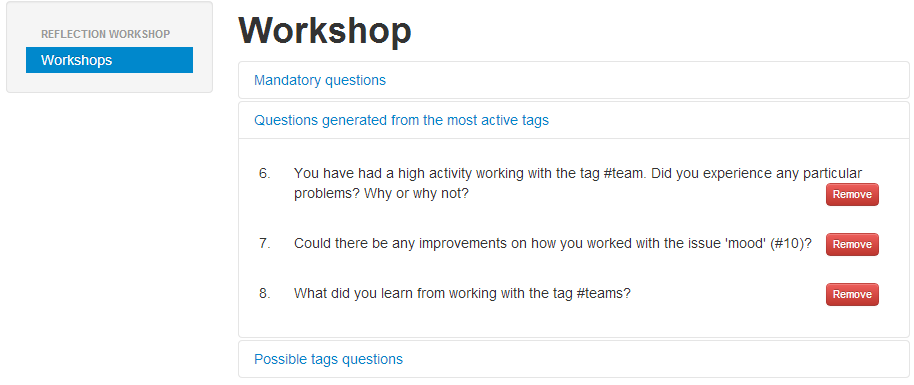
\includegraphics[width=\textwidth]{questionsgenerated}
\caption{PeacefulBanana - Workshop questions related to the most active tags}
\end{figure}

The questions are generated based on the most active tags on your team for the period the workshop spans. If you do not wish to keep any of these questions simply click the \textit{Remove} button. This will move the questions down to the \textit{Possible tag questions} tab.

\subsubsection*{Possible tag questions}
This tab contains all tags related to your teams current chosen workshop, in a descending order based on number of times the tag has been referenced in a commit. Clicking any of these tags will auto-generate a relevant question regarding this tag, and move it to the tab above. This allows you to quickly add and remove questions to your workshop. 
\begin{figure}[h!]
\label{questionsgenerated}
\centering
	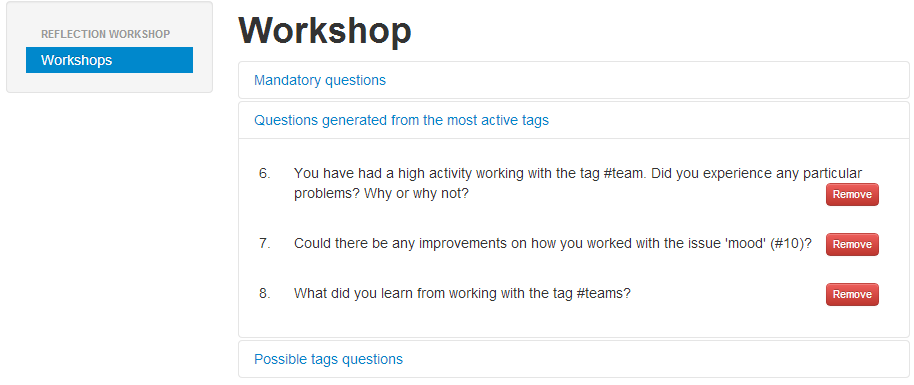
\includegraphics[width=\textwidth]{questionsgenerated}
\caption{PeacefulBanana - List of tags to generate questions from}
\end{figure}

\subsection{Summary}
\begin{enumerate}
\item Register in the PeacefulBanana application. Remember to check your email in order to complete the registration. 
\item Set an active team in the \textit{Team} tab. If there is no team, the team leader needs to create it. 
\item Wait for the GitHub sync to complete, you will be notified when the process is completed. Be aware that this might take a while if this is your first time syncing with the server.
\item You are now ready to complete your daily notifications or explore the app on your own and with your team. \\ Happy Reflecting
\end{enumerate}
\subsubsection*{Useful Links}
PeacefulBanana web-application: \url{http://goo.gl/JaUUg}
\begin{figure}[h!]
\label{logoappendix}
\centering
	
\includegraphics[width=\textwidth]{logo}
\end{figure}



